\documentclass{article}
\usepackage{graphicx} % Required for inserting images
\usepackage{amsmath, bm, mathtools, amsfonts, amssymb}
\usepackage{xcolor}
\usepackage{adjustbox} 
\usepackage{hhline}

\newcommand{\diff}{\mathop{}\!\mathrm{d}}

\usepackage{tikz}
\usetikzlibrary{decorations.pathreplacing,calligraphy}
\usetikzlibrary{positioning}
\usetikzlibrary{positioning,shapes.symbols,fit}
\tikzset{
	roundnode2/.style={circle, draw=green!50!blue, very thick, minimum size=9mm}
}
%\usetikzlibrary{shapes, arrows, calc, arrows.meta, fit, positioning}
%\usetikzlibrary{arrows.meta}
\tikzset{
	roundnode/.style={circle, draw=green!50!blue, fill=green!60!blue, very thick, minimum size=7mm},
	rectnode/.style={rectangle, draw=green!50!blue, very thick, minimum size=8.5mm},
	mydotted/.style = {dash pattern=on 6.1pt off 7pt}
}


%\usepackage[backend=bibtex,style=numeric,natbib=true,maxbibnames=5,giveninits=true]{biblatex}
\usepackage[backend=bibtex,style=numeric,natbib=true,maxbibnames=5,giveninits=true]{biblatex}
\newcommand*{\bibtitle}{References}
\DeclareNameAlias{default}{last-first}
\addbibresource{bib.bib}

\title{AffinePaper}
\author{Lennart }
\date{November 2025}

\begin{document}

\maketitle

\section{Introduction}
\begin{itemize}
    \item Hierarchical Bayesian modelling MTC Method
    \item Forward model ozone limb-sounding as linear inverse problem
    \item marginal and full conditional posterior explicitly formulated
    \item Marginal Posterior on Grid gives full posterior mean of ozone for free
    \item samples from full conditional posterior via IRT and Gibbs sampling
    \item sample-based affine map
    \item full posterior mean and sample-based variance do not capture second ozone peak
    \item All programming and analysis in this thesis are done in Python, and the reported computation times are taken on a MacBook Pro from 2019 with a 2.4 GHz quad-core Intel i5 processor.
\end{itemize}
\section{Linear inverse Problem --  Hierarchical Bayesian Modelling}
\label{sec:BayesIntro}
First the concept of hierarchical Bayesian modelling is introduced.
Assume we observe some data
\begin{align}
	\bm{y} = \bm{A} \bm{x} + \bm{\eta},
	\label{eq:NonLinDat}
\end{align}
based on a linear forward model $\bm{A}$ an unknown parameter vector $\bm{x}$ and some additive random noise $\bm{\eta}$.
Naturally, due to the noise, the observation process in Eq. \ref{eq:NonLinDat} is a random process.
Hence, in Bayesian modelling, the aim is to determine a probability distribution over the parameter $\bm{x}$ given some data $\bm{y}$.
Further, a hierarchical Bayesian model incorporates (auxiliary) hyper-parameters $\bm{\theta}$.
Within a Bayesian approach all unknown hyper-parameters and parameters are treated as random variables \cite[Chapter 3]{kaipio2005statinv}.

According to Bayes' theorem, the joint posterior distribution over the parameters $\bm{x}$ and the hyper-parameter $\bm{\theta}$ is given as
\begin{align}
	\pi(\bm{x},\bm{\theta}|\bm{y}) = \frac{ \pi(\bm{y} | \bm{x}, \bm{\theta} ) \pi(\bm{x}, \bm{\theta})}{\pi(\bm{y})} \propto \pi(\bm{y} | \bm{x}, \bm{\theta} ) \pi(\bm{x}, \bm{\theta}) \, ,
\end{align}
with finite and non-zero $\pi(\bm{y})$.
The likelihood function $\pi(\bm{y}|\bm{x},\bm{\theta})$ is defined by the nature of the noise and the noise-free data $\bm{A}\bm{x}$, which we read as the distribution over $\bm{y}$ conditioned on $\bm{x}$ and $\bm{\theta}$.
Here $\bm{\theta}$ describe multiple hyper-parameters, e.g.~the noise precision so that $\bm{\eta} \sim \pi_{\bm{\eta}}(\cdot|\bm{\theta})$, where $\sim$ reads as ``is distributed as''.
Further, $\bm{\theta}$ may account for some physical properties of $\bm{x}$ such as the smoothness (see Sec.~\ref{sec:BayModel}).
Because all unknown parameter are treated as random variables the joint prior distribution is introduced as $\pi(\bm{x}, \bm{\theta}) = \pi(\bm{x}|\bm{\theta}) \pi(\bm{\theta})$ with the parameter prior distribution $\pi(\bm{x}|\bm{\theta})$ and the hyper-prior distribution $\pi(\bm{\theta})$.
Choosing these prior distributions is ultimately a modeller's choice and is crucial, as those shall be as uninformative as possible for regions in hyper-parameter and parameter space where the data is informative.
If the data is uninformative, the prior distributions can be informative and may represent a rather restrictive range of (physically) feasible hyper-parameters and parameters.

We can write the hierarchical model as:
\begin{subequations}
	\begin{align}
		\bm{y} |  \bm{x},\bm{\theta}  &\sim \pi(\bm{y} | \bm{x}, \bm{\theta} ) \\
		\bm{x}| \bm{\theta}   &\sim \pi(\bm{x}|\bm{\theta})   \\
		\bm{\theta}   &\sim \pi(\bm{\theta} ) \, .
	\end{align} 
\end{subequations}
Usually, the objective is to calculate the expectation of a function $h(\bm{x})$, which is defined as
\begin{align}
	\text{E}_{\bm{x},\bm{\theta}|\bm{y}} [h(\bm{x})] =  \int \int   h(\bm{x}) \,  \pi(\bm{x}, \bm{\theta} | \bm{y} ) \, \diff \bm{x}  \, \diff \bm{\theta}  \label{eq:expPos} \, .
\end{align}
\subsection{Marginal and then Conditional Method}
\label{subsec:TheoMTC}
Characterising the posterior distribution or quickly generating a representative sample set from the posterior distribution often presents a significant challenge. 
This is mainly due to the strong correlations that usually exist between the parameters $\bm{x}$ and hyper-parameters $\bm{\theta}$, as discussed by Rue and Held in~\cite{rue2005gaussian}.

Depending on the problem and the available model it is beneficial to factorise the joint posterior distribution
\begin{align}
	\pi(\bm{x}, \bm{\theta} |  \bm{y}) = \pi(\bm{x} |  \bm{\theta}, \bm{y}) \, \pi(\bm{\theta} |   \bm{y}) \label{eq:MTC}
\end{align}
into the full conditional posterior $\pi(\bm{x} |  \bm{\theta}, \bm{y})$ over the latent field $\bm{x}$ and the marginal posterior $ \pi(\bm{\theta} |   \bm{y})$ over hyper-parameter $\bm{\theta}$.
This approach, known as the marginal and then conditional (MTC) method~\cite{fox2016fast}, is particularly advantageous when $\bm{x}\in \mathbb{R}^n$ is high-dimensional, while $\bm{\theta}$ is low-dimensional and the evaluation of the marginal posterior
\begin{align}
	\pi(\bm{\theta} |   \bm{y}) =  \frac{ \pi(   \bm{y} | \bm{x},\bm{\theta})  \pi( \bm{x} | \bm{\theta} )  \pi(\bm{\theta}) }{ \pi(\bm{x} | \bm{\theta} ,   \bm{y})   \pi( \bm{y})} \propto \frac{ \pi(   \bm{y} | \bm{x},\bm{\theta})  \pi( \bm{x} | \bm{\theta} )  \pi(\bm{\theta}) }{ \pi(\bm{x} | \bm{\theta} ,   \bm{y}) } \label{eq:margGen}\, 
\end{align}
as in~\cite[Lemma 2]{fox2016fast} is relatively cheap.

Applying the law of total expectation~\cite{champ2022generalizedlawtotalcovariance}, Eq.~\eqref{eq:expPos} becomes
\begin{align}
	\mathbb{E}_{\bm{x} ,\bm{\theta}  |\bm{y}} [h(\bm{x})] &= \int \int   h(\bm{x}) \pi(\bm{x} |  \bm{\theta}, \bm{y}) \, \diff \bm{x} \,  \pi(\bm{\theta} |   \bm{y}) \, \diff \bm{\theta} \\
	&= \int \mathbb{E}_{\bm{x} |  \bm{\theta}, \bm{y}} \left[ h(\bm{x}) \right] \, \pi(\bm{\theta} |  \bm{y}) \, \diff \bm{\theta}\label{eq:2fullCond} \\
		&= \mathbb{E}_{\bm{\theta} |  \bm{y}} \left[ \mathbb{E}_{\bm{x} |  \bm{\theta}, \bm{y}} [h(\bm{x})] \right] \, .
	\label{eq:fullCond}
\end{align}
In the case of a linear-Gaussian hierarchical Bayesian model, both the marginal distribution $\pi (\bm{\theta}| \bm{y})$ 
and the inner expectation $\mathbb{E}_{\bm{x} |  \bm{\theta}, \bm{y}} \left[ h(\bm{x}) \right]$ are well defined (see Sec.~\ref{sec:BayModel}).
If the integral in Eq.~\ref{eq:2fullCond} is expensive to calculate  sample-based methods may be used to calculate the expectations in 
Eq.~\eqref{eq:2fullCond}.
To produce a samples $\{ (\bm{x}, \bm{\theta})^{(1)}, \dots, (\bm{x}, \bm{\theta})^{(k)}, \dots, (\bm{x}, \bm{\theta})^{(N)} \} \sim \pi(\bm{x}, \bm{\theta} |  \bm{y}) $ one needs an independent an sample from $\bm{\theta}^{(k)} \sim \pi(\bm{\theta} |  \bm{y})$ first and then draw a sample from the full conditional posterior $\bm{x}^{(k)} \sim \pi(\bm{x} | \bm{\theta}^{(k)}  , \bm{y})$.


\section{The Forward Model}
\label{ch:formodel}
Here we present the forward model to which we apply the methodology.
The forward model describes a Limb-sounder measuring thermal radiation of ozone to determine the atmospheric ozone concentration.
We follow the MIPAS handbook~\cite{mipas2000handbook} and simulate data according to an idealised cloud-free atmosphere in local thermodynamic equilibrium, assuming a measurement instrument with infinite spectral resolution and no pointing errors.
This is a simplified forward model.
No other instrument-specific details such as sensor area or antenna response are included because they are not available to us. 

\begin{figure}[ht!]
	\centering
	\input{LIMB.pdf_tex}
	\caption[Schematic of measurement and analysis geometry.]{Schematic of measurement and analysis geometry, not to scale.
		The stationary satellite, at a constant height $h_\text{sat}$ above Earth, takes $m$ measurements along its line-of-sight defined by the line $\Gamma_j$.
		Each measurement has a pointing angle $\phi_j$ and a tangent height $h_{\ell_j}$, $j=1,2,\dots,m$ defined as the closest distance of $\Gamma_j$ to the Earth's surface.
		Between $h_{L,0} \approx 7$km and $h_{L,n} \approx 83$km, the atmosphere is discretised into $n$ layers as illustrated by the solid green lines.}
	\label{fig:LIMB}
\end{figure}
As displayed in Fig.~\ref{fig:LIMB}, a satellite at a constant height $h_{\text{sat}}$ is pointing through the atmosphere (limb-sounding) to measure thermal radiation of ozone.
For each measurement $j=1,2,\ldots,m$, the tangent height $h_{\ell_j}$ and the corresponding line-of-sight $\Gamma_j$ are defined.
Additionally, we introduce the pointing angle $0 \leq \phi_j < \phi_{\text{max}}$, so that if $\phi = 0 \text{arc sec}$ the satellite points at $h_{L,0}$ and for a pointing angle $\phi_{\text{max}}$ at $h_{L,n}$.
Further, the atmosphere is discretised into $n$ layers defined by height values $h_{L,i-1} < h_{L,i}$ with respect to the surface of the Earth, for $i = 1, \dots, n$.
More specifically, the $i$-th layer is defined by two spheres around the centre of the Earth with radii $ r_0 + h_{L,i-1} $ and $r_0 + h_{L,i}$, where $r_0$ is the Earth's radius.
Within a layer the signal is constant, whereas above $h_{L, n}$ and below $h_{L,0} $ no signal can be obtained.


\subsection{Radiative Transfer Equation}
\label{sec:RTE}
One noise-free measurement of thermal radiation emitted by gas molecules within the atmosphere is described by the radiative transfer equation (RTE)~\cite{mipas2000handbook}
\begin{align}
	\label{eq:RTE} 
	  \int_{\Gamma_j}  B(\nu,T) k(\nu, T)   \frac{p(r)}{k_{\text{B}} T(r)}  x(r)  \tau(r) \text{d}r \,  \\
\text{with } \,	\tau(r) = \exp{ \Bigl\{ - \int^{r}_{r_\text{obs}}  k(\nu, T)   \frac{p(r^{\prime})}{k_B T(r^{\prime})}  x(r^{\prime}) \text{d}r^{\prime} \Bigr\} } \, \label{eq:absRTE} .
\end{align}
This is a path integral along the satellite's straight line of sight $\Gamma_j$ with the ozone volume mixing ratio (VMR) $x(r)$ at distance $r$ from the satellite, at the wave number $\nu$.
Within the atmosphere, the number density $p(r) / (k_{\text{B}} T(r))$ of molecules is dependent on the pressure $p(r)$, the temperature $T(r)$, and the Boltzmann constant $k_{\text{B}}$.
The factor $\tau(r)\leq 1$ accounts for re-absorption of the radiation along the line-of-sight, which makes the RTE non-linear.
The absorption constant is given as
\begin{align}
	k(\nu, T) = L(\nu, T_{\text{ref}}) \frac{Q(T_{\text{ref}})}{Q(T)} \frac{ \exp{\{ - c_2 E^{\prime \prime} / T\}} }{\exp{\{ - c_2 E^{\prime \prime} / T_{\text{ref}} \}}} \frac{ 1- \exp{\{ - c_2 \nu  / T \}} }{1 - \exp{\{ - c_2 \nu / T_{\text{ref}} \}}}
\end{align}
with Planck's constant $h$ and speed of light $c$.
The line intensity $L(\nu, T_{\text{ref}})$ at reference temperature $T_{\text{ref}} =296K $, the lower-state energy $ E^{\prime \prime} $ in $\text{cm}^{-1}$ of the targeted transition and the second radiation constant $c_2\coloneqq hc/k_{\text{B}} \approx 1.44\text{cmK}$ are provided by the HITRAN database~\cite{gordon2022hitran2020}.
The total internal partition function is given as
\begin{align}
	Q(T )= g^{ \prime} \exp{\{ - \frac{ c_2 E^{ \prime} }{T}\}} + g^{\prime \prime} \exp{\{ - \frac{ c_2 E^{\prime \prime} }{T}\}} \, ,
\end{align}
with the statistical weight $ g^{\prime \prime}$ for the lower and $ g^{ \prime}$ for the upper energy state (also called the degeneracy factors) accounting for the molecule's non-rotational and rotational energy states (see also~\cite{vsimevckova2006einstein}), and the upper state energy $E^{ \prime} = E^{ \prime\prime} + \nu$.
Under the assumption of local thermodynamic equilibrium (LTE), the black body radiation acts as a source function
\begin{align}
	B(\nu,T)   = \frac{2 h c^2 \nu^3}{\exp{\{\frac{c_2\nu}{ T}\}}-1}\, .
\end{align}
For fundamentals on the RTE, we recommend~\cite[Chapter 1]{rybicki2000rte}, and for a more comprehensive model, we refer to \cite{read2006forwardModel}.

When simulating data, we assume an idealised limb-sounder.
Since the measurement device has a negligible frequency window, the line broadening around $\nu$ for the calculations of $L(\nu, T_{\text{ref}})$ is neglected.
Normally, this is modelled as the convolution of the normalised Lorentz profile (collisional/pressure broadening) and the normalised Doppler profile (thermal broadening)~\cite{mipas2000handbook}.
Additionally, we target one specific molecule and calculate $k(\nu, T)$ accordingly.
Usually, this would involve a summation over the individual absorption constants for multiple radiating molecules weighted by their respective VMR~\cite{mipas2000handbook}.


\subsection{Simulated Data and Ground Truth}
\label{sec:SimDat}
As the ground truth for our methodology, we consider an ozone profile at distinct pressure values generated from some data~\cite{MLSdata} of the MLS on the Aura satellite within the Antarctic region.
This ozone profile has a peak in the middle atmosphere and a second peak at higher altitudes, see Fig.~\ref{fig:OzonSampl}, which seems to be a typical nighttime profile~\cite{Lee2020NightOzone}.
For more information on the processes within the atmosphere for ozone, we refer to~\cite{Lee2020NightOzone}.

We can relate the height $h$ and the pressure values $p$ via the hydrostatic equilibrium equation
\begin{align}
	\text{d}(\log p) = \frac{\text{d}p}{p} = \frac{- g M}{R^* T} \text{d} h \, .\label{eq:hydr}
\end{align}
Here the acceleration due to gravity is $g$, the universal gas constant is $R^* = 8.31432 \times 10^{-3} \text{Nm} / \text{kmol} / \text{K}$ and the mean molecular weight of the air is $M = 28.97 \text{kg/kmol}$, as in~\cite{atmosphere1976us}.
To enable efficient calculation of the RTE we discretise the atmosphere as in Fig.~\ref{fig:LIMB}.
Then the ozone VMR $\bm{x} =\{x_1,x_2,\ldots,x_n\} \in \mathbb{R}^{n}$, pressure $\bm{p} =\{p_1,p_2,\ldots,p_n\} \in \mathbb{R}^{n}$ and temperature $\bm{T} =\{T_1,T_2,\ldots,T_n\} \in \mathbb{R}^{n}$, as well as all other height dependent parameters, are discretised profiles with constant values between the heights $h_{L,i-1} \leq h < h_{L,i}$, for each layer $i = 1,\dots, n$.
The hydrostatic equilibrium equation for the discretised atmosphere is
\begin{align}
	h_{L,i} =  h_{L,i-1} - \frac{\Delta p R^* T_{i-1}  }{p_{i-1}  g_{i-1} M} \, 
\end{align}
with $\Delta p = p_{i} - p_{i-1}$ and $T_{i-1} = T(h_{i-1})$ as in Eq.~\ref{eq:tempFunc} (see also~\cite{Carlotti99,Ridolfi00}), for $i = 1,\dots, n$.
At sea level $h = 0$km the mean pressure is $p_0 = 1013.25$hPa and the mean temperature is $T_0 = 288.15$K~\cite{atmosphere1976us}.
The acceleration due to gravity is
\begin{align}
	g_i = g_0 \Bigg( \frac{r_0}{r_0 + h_{L,i}} \Bigg) \, ,
\end{align}
where the polar radius of the Earth is $r_0 \approx 6356 \, \text{km}$, the gravitation at sea level is $g_0 \approx 9.81 \text{m}/\text{s}^2$.
For a ground truth temperature profile we follow~\cite{atmosphere1976us} and form the temperature function
\begin{equation}
	\label{eq:tempFunc}
	T(h) = \adjustbox{max width=0.825\textwidth}{$\begin{dcases*}
			T_0 &, \text{$h  = 0$}\\
			T_0 + a_0 h   &, \text{$0 \leq h < h_{T,1}$}\\
			T_0 + a_0 h_{T,1} &, \text{$h_{T,1} \leq  h < h_{T,2}$}\\
			T_0 + a_0 h_{T,1} + a_1 (h_{T,2}   - h_{T,1})  + a_2 (h   - h_{T,2})  &, \text{$h_{T,2} \leq h < h_{T,3}$}\\
			T_0 + a_0 h_{T,1} + a_1 (h_{T,2}   - h_{T,1})   & \\
			\hphantom{{} T_0 } + a_2 (h_{T,3}   - h_{T,2}) + a_3 (h   - h_{T,3}) &, \text{$h_{T,3} \leq h < h_{T,4}$}\\
			T_0 + a_0 h_{T,1} + a_1 (h_{T,2}   - h_{T,1})  & \\
			\hphantom{{} T_0 }+ a_2 (h_{T,3}   - h_{T,2})  + a_3 (h_{T,4}   - h_{T,3}) + a_4 (h   - h_{T,4}) &, \text{$h_{T,4} \leq h < h_{T,5}$}\\
			T_0 + a_0 h_{T,1} + a_1 (h_{T,2}   - h_{T,1})   & \\
			\hphantom{{} T_0 } + a_2 (h_{T,3}   - h_{T,2}) + a_3 (h_{T,4}   - h_{T,3}) + a_4 (h_{T,5}   - h_{T,4})& \\
			\hphantom{{} T_0 }  + a_5 (h   - h_{T,5}) &, \text{$h_{T,5} \leq h < h_{T,6}$}\\
			T_0 + a_0 h_{T,1} + a_1 (h_{T,2}   - h_{T,1})    &\\
			\hphantom{{} T_0}  + a_2 (h_{T,3}   - h_{T,2}) + a_3 (h_{T,4}   - h_{T,3}) + a_4 (h_{T,5}   - h_{T,4}) &\\ 
			\hphantom{{} T_0} + a_5 (h_{T,6}   - h_{T,5}) + a_6 (h   - h_{T,6})   &, \text{$h_{T,6} \leq h \lesssim  86$}
		\end{dcases*}$}\\
\end{equation}
with gradient and height values in Tab.~\ref{tab:tempGrad} provided by~\cite{atmosphere1976us}.
This function describes the mean temperature in the atmosphere with various height-depending gradients according to the different atmospheric layers.
This holds up to a geometric height of $86$km, where we ignore a $0.04\%$ non-linear change in $M$ from $80$km to $86$km.
\begin{table}
	\centering
	\begin{tabular}{ |c||c|c|  }
		\hline
		subscript $i$ & geometric height $h_{T,i}$ in km&gradient $a_i$\\
		\hhline{|=||=|=|}
		0& 0 & -6.5\\
		1& 11 & 0\\
		2& 20.1& 1\\
		3& 32.2& 2.8\\
		4& 47.4& 0\\
		5& 51.4& -2.8\\
		6& 71.8& -2\\
		\hline
	\end{tabular}
	\caption[Height depending temperature gradients]{Definition of height depending temperature gradients.}
	\label{tab:tempGrad}
\end{table}

We target ozone at a frequency of $235.71$GHz, which lies within the region where the MLS observes ozone~\cite{livesey2008ozonecarbonmono, waters2006earth}.
The corresponding wave number is $\nu = 7.86\text{cm}^{-1}$.
The absorption constant $k(\nu,T)$ is calculated as in Eq.~\ref{eq:absRTE}, following the high-resolution transmission (HITRAN) database~\cite{gordon2022hitran2020}.
The HITRAN database provides the line intensity $L(\nu,T_{\text{ref}})$ for the isotopologue $\prescript{16}{}{\text{O}}_3$ with the AFGL Code 666.

To compute a data vector, we define an atmosphere between $h_{L,0} = 6.9$km and $h_{L,n} = 83.3$km with $n = 45$ equidistant layers and a satellite fixed at a height of $h_{\text{sat}} = 500$km (see Fig.~\ref{fig:LIMB}).
We measure $m=30$ times between heights of $\approx 7$km and $\approx 68$km with pointing accuracy $175  \text{arc sec}$ and equidistant spaced pointing angles
\begin{align*} 
		\phi_j  =  (j-1) 175 \text{arc sec} ,  \qquad  \text{for } j = 1, \dots, 30\, .
\end{align*}
Above $\approx 68$km the data is noise dominated (see Fig.~\ref{fig:Data}), hence no measurement are taken in larger altitudes.
Each pointing angle $\phi_j$ defines a path $\Gamma_j$ (see Fig.~\ref{fig:LIMB}).
The corresponding path integrals in Eq.~\ref{eq:RTE} and Eq.~\ref{eq:absRTE} are evaluated using the trapezoidal rule and define the non-linear forward model $\bm{A}(\bm{x},  \bm{p},\bm{T})   \in \mathbb{R}^{m}$ for the set of $m$ noise-free measurements.
Here, each entry $A_{j}$ of $\bm{A}(\bm{x},\bm{p},\bm{T})\in \mathbb{R}^{m}$ includes multiple evaluations of the integral in Eq.~\ref{eq:absRTE} to calculate the absorption $\tau(r)$.
For brevity we denote the non-linear forward model as $\bm{A}(\bm{x}) \coloneqq \bm{A}(\bm{x},  \bm{p},\bm{T})$.
The simulated data vector
\begin{align}
	\bm{y} = \bm{A}(\bm{x}) + \bm{\eta}\, 
\end{align}
includes an additive identically-distributed Gaussian noise vector $\bm{\eta} \sim \mathcal{N}(0,\gamma^{-1} \bm{I})$.
The noise precision is chosen so that the signal-to-noise ratio (SNR) is approximately $150$.
The SNR is defined as
\begin{align}
	\text{SNR} \coloneqq \frac{\max(y)}{\text{STD noise}} = \frac{\text{peak signal}}{\text{RMS noise}} \label{eq:SNR} \, ,
\end{align}
where STD noise is the standard deviation of the noise.
An SNR of 150 is similar to~\cite{Froidevaux2008snrozone}, where a signal with a maximal spectral intensity of around $100\text{K}$ and a noise range of $0.4$ to $1.6\text{K}$ is reported.

By neglecting the absorption (e.g., set $\tau = 1$ in Eq.~\eqref{eq:absRTE}) the RTE is linearised.
This denotes the linear forward model matrix $\bm{A}_L\in \mathbb{R}^{m\times n}$.
The integral in Eq.~\eqref{eq:RTE} is evaluated using the trapezoidal rule and enables matrix-vector multiplication $\bm{A}_L \bm{x}$ to compute noise-free linear data.
Since neglecting the absorption changes the measurements only slightly (about $1\%$, see Sec.~\ref{sec:affine}), we classify the inverse problem as a weakly non-linear inverse problem.
Note that the methods used here will work with different SNRs or other frequencies.

\section{Linear-Gaussian Hierarchical Bayesian Model}
\label{sec:BayModel}
Here this inverse problem is treated as a linear inverse problem by neglecting the absorption term in the RTE (see Eq.~\ref{eq:RTE}).
The reader is guided through the process of setting up a hierarchical Bayesian frameworka and establishing a choice of prior distributions.
Applying the MTC scheme, we explicitly formulate the respective posterior distributions.
A directed acyclic graph (DAG) is used to visualise conditional dependencies between hyper-parameters and the parameter (see Fig.~\ref{fig:DAGO3}), as well as how distributions progress through to an observation (square box). 
We plot statistical dependencies as solid arrows and deterministic dependencies as dotted arrows.

\begin{figure}[htb!]
	\centering
	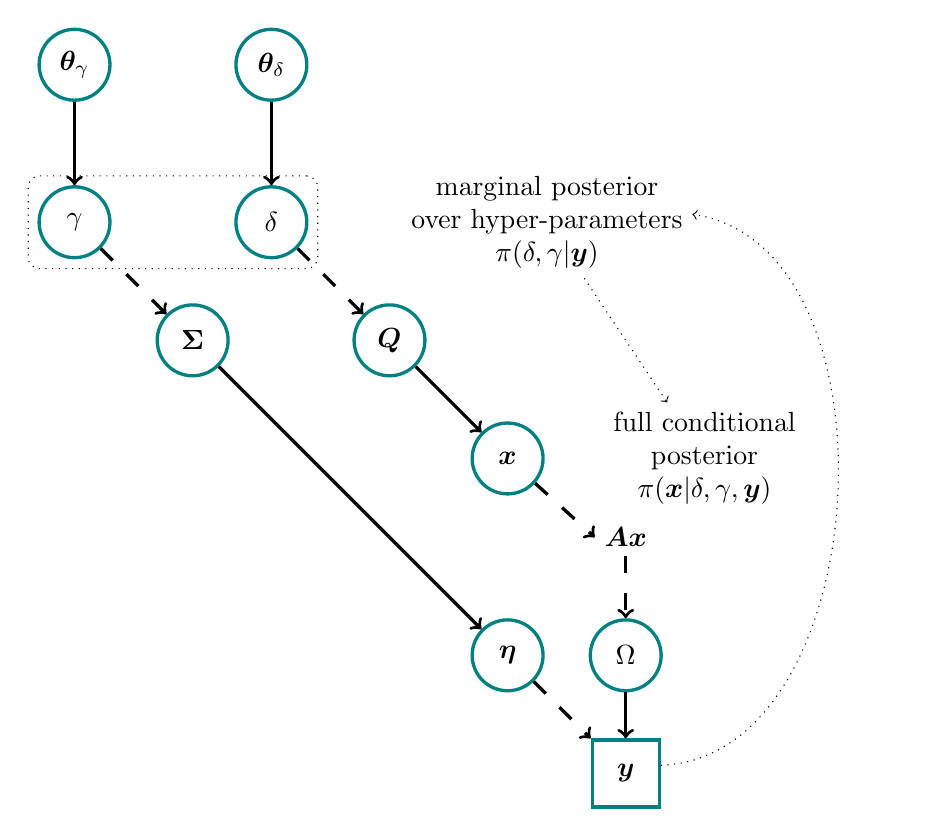
\begin{tikzpicture}
		%box/.style = {draw, thick, minimum width=2.5cm, minimum height=1cm},
		every edge/.style = {draw, -latex, thick} % <---
		\node[roundnode2] at (-4,6.5) (Q)     {$\bm{Q}$};
		\node[roundnode2] at (-2.5,5) (x)     {$\bm{x}$};
		\node[align=center] at (-1,4) (A)    {$\bm{A} \bm{x}$};
		\node[roundnode2] at (-1,2.5) (u)    {$\Omega$};
		\node[rectnode] at (-1,1) (y)    {$\bm{y}$};
		\node[roundnode2] at (-2.5,2.5) (e)    {$\bm{\eta}$};
		\node[roundnode2] at (-6.5,6.5) (S)    {$\bm{\Sigma}$};
		\node[roundnode2] at (-8,8) (s)    {$\gamma$};
		\node[roundnode2] at (-5.5,8) (d)    {$\delta$};
		
		\node[roundnode2] at (-8,10) (shyp)    {$\bm{\theta}_{\gamma}$};
		\node[roundnode2] at (-5.5,10) (dhyp)    {$\bm{\theta}_{\delta}$};
		%Lines
		\draw[->, very thick] (S) -- (e);
		\draw[->, mydotted, very thick] (s) -- (S);
		\draw[->, mydotted, very thick] (e) -- (y);
		\draw[->, very thick] (u.south) -- (y);
		\draw[->, mydotted, very thick] (A) -- (u);
		\draw[->, mydotted,  very thick] (x) -- (A.west);
		\draw[->, very thick] (shyp) -- (s);
		\draw[->, very thick] (dhyp) -- (d);
		
		
		\draw[->, mydotted, very thick] (d) -- (Q); 
		
		\draw[->, very thick] (Q) -- (x); 
		%\node[align=center] at (0,4) (f3) {$= \bm{A}$};
		%\node[align=center] at (0.25,3.95) (f3) {$\approx \bm{M A}_L$};
		\node[align =center] at (-2,8) (T1) {marginal posterior \\ over hyper-parameters \\ $\pi(\delta,\gamma  | \bm{y})$};
		\node[align =center] at (0,5) (T2) {full conditional \\ posterior \\ $\pi( \bm{x} | \delta,\gamma, \bm{y})$ };
		
		%\node[align =center] at (-2.5,10) (T3) {hyper-prior distributions \\ $\pi( \delta, \gamma)$ };
		
		\node[fit=(s)(d),draw,dotted,black, rounded corners] {};
		\draw[->,dotted] (y) edge[bend right=85] (T1);  
		\draw[->,dotted] (T1) -- (T2); 
		
	\end{tikzpicture} 
	\caption[Directed acyclic graph for ozone retrieval and MTC scheme.]{DAG for visualisation of the hierarchical modelling process and the conditional dependency between the parameter and the hyper-parameters. The hyper-parameter $\gamma$ deterministically (dotted line) sets the noise covariance $\bm{\Sigma} = \gamma^{-1}\bm{I}$, which then describes the random (solid line) noise vector $\bm{\eta} \sim \mathcal{N}(0, \gamma^{-1}\bm{I})$.
		The hyper-parameter $\delta$ determines (dotted line) the prior precision matrix $\bm{Q} = \delta \bm{L}$ for the normally distributed (solid line) prior $\bm{x}| \delta \sim \mathcal{N}(0, (\delta \bm{L})^{-1})$, where $\bm{L}$ is a graph Laplacian, see Eq.~\ref{eq:GLapl}.
		The hyper-prior distributions (solid line) $\pi(\delta, \gamma)$ are defined by $\bm{\theta}_{\gamma}$ and $\bm{\theta}_{\delta}$.
		Through a linear forward model $\bm{A}$, we generate a space $\Omega$ of all measurable noise-free data $\bm{A}\bm{x}$.
		From $\Omega$ we randomly observe a data set $\bm{y}$ including some added noise $\bm{\eta}$.
		Within the MTC scheme, we evaluate the marginal posterior over the hyper-parameters $\pi(\gamma, \delta | \bm{y})$ first and then the full conditional posterior $\pi(\bm{x}|\delta,\gamma,\bm{y})$. This breaks the correlation structure of $\delta$ and $\gamma$, and $\bm{x}$, and allows us to evaluate the marginal posterior independently of $\bm{x}$.}
	\label{fig:DAGO3}
\end{figure}
In this section, we set up the hierarchically-ordered linear-Gaussian Bayesian framework to determine the ozone posterior distribution, conditioned on ground truth temperature and pressure.
For now the linear forward model matrix is defined as $\bm{A} \coloneqq \bm{A}_L$ by neglecting the absorption term in the RTE.
The distributions that define the hierarchical Bayesian model are:
\begin{subequations}
	\begin{align}
		\bm{y} |  \bm{x},\delta, \gamma  &\sim \mathcal{N}(\bm{A} \, \bm{x}, \gamma^{-1} \bm{I}) \label{eq:likelihoodAppl} \\
		\bm{x}| \delta  &\sim \mathcal{N}(\bm{0}, (\delta \bm{L})^{-1} ) \label{eq:priorXAppl} \\
		\delta  &\sim \mathcal{T}(\alpha_{\delta}, \beta_{\delta})\label{eq:priorDelAppl} \\
		\gamma  &\sim \mathcal{T}(\alpha_{\gamma}, \beta_{\gamma})\label{eq:priorGamAppl} \, .
	\end{align} 
\end{subequations}
Assuming Gaussian noise $\bm{\eta} \sim \mathcal{N}(0, \gamma^{-1} \bm{I})$, the likelihood function is a normal distribution with mean $\bm{A} \bm{x}$ and covariance matrix $\gamma^{-1} \bm{I}$.
We define a normal prior-distribution $\pi(\bm{x}|\delta)$ with zero mean and precision matrix $\delta \bm{L}$, where $\delta$ is a smoothness hyper-parameter and $\bm{L}$ is a discrete approximation to the second derivate operator (see Eq.~\ref{eq:GLapl}).
Here the hyper-prior distributions $\pi(\delta)$ and $\pi(\gamma)$ are Gamma distributions with shape $\alpha$ and rate $\beta$.

We can visualise this hierarchical structure and the conditional dependencies between hyper-parameters and parameters through a DAG, as in Fig.~\ref{fig:DAGO3}.
The hyper-parameter $\gamma$ sets the noise covariance deterministically (dotted line), but is itself statistically (solid line) defined by the hyper-prior distribution $\pi(\gamma)$.
This is a Gamma distribution, where $\bm{\theta}_{\gamma}$ determines the shape and rate of $\pi(\gamma)$.
Similarly $\bm{\theta}_{\delta}$ defines the Gamma distribution $\pi(\delta)$.
%The prior distribution $\pi(\bm{x}|\delta)$ is a normal distribution with zero mean and precision matrix $\bm{Q}(\delta) =\delta \bm{L}$.
Through the linear forward model the space $\Omega$ is determined by all measurable noise-free data sets $\bm{A}\bm{x}$.
From that space we observe (square box) a data set $\bm{y}$ including some additive noise $\bm{\eta}$.

Given that data, we ``reverse the arrows'' to determine the posterior distribution $\pi(\bm{x}, \delta, \gamma |\bm{y})$ over the parameter $\bm{x}$ and the hyper-parameters $\delta$ and $\gamma$.
%Since noise is a random process with a defined distribution, the posterior distribution $\pi(\bm{x}|\bm{y})$ is well defined.
Usually, due to underlying correlation structures between the parameter and the hyper-parameters, evaluating this posterior poses a signifiant challenge.
The MTC scheme breaks this correlation and provides the marginal posterior $\pi(\delta, \gamma | \bm{y})$ first and then the full conditional posterior $\pi(\bm{x}|\delta, \gamma,\bm{y})$.



\subsubsection{Prior Modelling}
\label{subsec:PriorModelO3}
Completing this Bayesian framework one has to define prior distributions over the hyper-parameters and parameters.
Ideally, we define the prior distributions as uninformative as possible, and include functional dependencies and physical properties.

By choosing a normally distributed prior $\pi(\bm{x}|\delta)$ with zero mean and no other restrictions, it is clear that our model does not take into account that ozone values cannot be negative.
The the precision matrix of that prior distribution is
\begin{align}
	\delta \bm{L} =
	\delta
	\begin{bmatrix}
		2 & -1 & & &  \\
		-1 & 2 & -1 & &   \\
		& \ddots & \ddots & \ddots &\\ 
		& & -1 & 2 & -1  \\
		& & & -1 & 2 
	\end{bmatrix} 
	\label{eq:GLapl} 
\end{align}
which is a discrete approximation to the second derivate operator with Dirichlet boundary condition and defines a 1-dimensional Graph Laplacian as in~\cite{wang2015graphs, fox2016fast}.
We reduce the dimension of $\bm{x}$ from $45$ to $n = 34$ by discarding every second ozone VMR over a height of $\approx47$km.
Doing that, while not changing $\bm{L}$ effectively induces a larger correlation between points at higher altitude.

For $\delta$ and $\gamma$ we pick relatively uninformative Gamma distributions so that \linebreak$\gamma \sim \mathcal{T}(\bm{\theta_{\gamma}}) \propto \gamma^{\alpha_\gamma -1 } \exp{( -\beta_\gamma \gamma) } $ and $\delta \sim \mathcal{T}(\bm{\theta_{\delta}})$ with $\bm{\theta_{\gamma}} = \{  \alpha_\gamma, \beta_\gamma\}  = \{ \alpha_\delta ,\beta_\delta\} = \bm{\theta_{\delta}} = (1,10^{-35})$ similar to \cite{fox2016fast}.
Because of those Gamma distributions, $\pi(\gamma | \lambda, \bm{y}) \sim \mathcal{T}(\cdot)$ is a Gamma distribution with $\lambda = \delta / \gamma $ and easy to sample from.


\subsection{Posterior Distribution}
\label{sec:FirstO3Post}
As explained in Sec.~\ref{subsec:TheoMTC}, we factorise the posterior
\begin{align}
	\pi( \bm{x}, \delta, \gamma| \bm{y}) \propto \pi(\bm{y}| \bm{x},\delta,\gamma) \pi( \bm{x},  \delta,\gamma)
\end{align}
into 
\begin{align}
	\pi( \bm{x},  \delta,\gamma| \bm{y}) =\pi( \bm{x}| \delta,\gamma, \bm{y})\pi( \delta,\gamma | \bm{y})
\end{align}
the marginal posterior $\pi(\delta ,\gamma| \bm{y})$ and full conditional posterior $\pi( \bm{x}| \delta,\gamma, \bm{y})$ (see Eq.~\ref{eq:MTC}).
%Fox and Norton call this method the marginal and then conditional method (MTC) \cite{fox2016fast}, where we break the correlation structure between $\bm{x}$ and $\gamma, \delta$ as illustrated in Fig. \ref{fig:RueHeld} by marginalising over $\bm{x}$.
As discussed in~\cite{fox2016fast}, for the linear-Gaussian case, $\bm{x}$ cancels in the marginal posterior over the hyper-parameters.
Following the MTC scheme, we characterise the marginal posterior first and then the full conditional posterior.

\subsubsection{Marginal Posterior}
\label{subsec:FirstMargPost}
For the hierarchical model specified in Eq.~\ref{eq:likelihoodAppl} to Eq.~\ref{eq:priorGamAppl}, the marginal posterior distribution over the hyper-parameters is given by
\begin{align}
	\pi( \lambda,\gamma  | \bm{y}) \propto &  \lambda^{n/2 + \alpha_{\delta}-1} \gamma^{m/2 + \alpha_{\delta} + \alpha_{\gamma}-1}   \exp{ \Bigl\{ - \frac{1}{2} g ( \lambda) - \frac{\gamma}{2} f ( \lambda) - \beta_{\delta} \lambda  \gamma - \beta_{\gamma} \gamma \Bigr\}},
	\label{eq:MargPostTheo}
\end{align}
with the regularisation parameter $\lambda = \delta / \gamma$, and
\begin{subequations}
	\begin{align}
		&f ( \lambda) = \bm{y}^T \bm{y} - (\bm{A}^T \bm{y})^T (\bm{A}^T  \bm{A} + \lambda \bm{L})^{-1} \bm{A}^T \bm{y}  \label{eq:fAppl} \, ,  \\
		&\text{and } g(\lambda) = \log \det (\bm{A}^T  \bm{A} + \lambda \bm{L}) \label{eq:gAppl} \, .
	\end{align}
\end{subequations}
Note that when changing variables from $\delta = \lambda \gamma$ to $\lambda$ the hyper-prior distribution changes to $\pi(\lambda | \gamma) \propto \lambda^{\alpha_{\delta}-1} \gamma^{\alpha_{\delta}} \exp{(- \beta_{\delta} \lambda  \gamma)} $, due to $\text{d}\delta / \text{d} \lambda = \gamma$.
Here, $\lambda$ is introduces as the regularisation parameter \cite{fox2016fast}.
Because of the chosen Gamma priors the conditional marginal posterior 
\begin{align}
	\gamma |  \lambda, \bm{y} &\sim \mathcal{T}\bigg( \frac{m}{2} + \alpha_\delta + \alpha_\gamma, \frac{1}{2} f (\lambda) + \beta_\gamma + \beta_\delta \lambda \bigg)\label{eq:GibbsStep}
\end{align} 
is a Gamma distribution.

\subsubsection{Full Conditional Posterior}
\label{subsec:firstCond}
As in \cite{SIMPSON201216}, consider the joint Gaussian distribution
\begin{align}
	\begin{pmatrix}
		\bm{x} \\
		\bm{y}
	\end{pmatrix}\sim \mathcal{N}\left[  \begin{pmatrix}
		\bm{\mu} \\
		\bm{A}\bm{\mu}
	\end{pmatrix},\begin{pmatrix}
		\bm{Q}_{\bm{\theta}} + \bm{A}^T \bm{\Sigma}_{\bm{\theta}}^{-1} \bm{A} & - \bm{A}^T \bm{\Sigma}_{\bm{\theta}}^{-1} \\
		\bm{\Sigma}_{\bm{\theta}}^{-1} \bm{A} & \bm{\Sigma}_{\bm{\theta}}^{-1} 
	\end{pmatrix}^{-1} \right] \, 	\label{eq:jointMultiGaus}
\end{align}
with $\bm{\Sigma}_{\bm{\theta}}^{-1} = \gamma \bm{I} $ and $\bm{Q}_{\bm{\theta}}  = \delta \bm{L} $ and $\bm{\mu} = \bm{0}$.
Then the full conditional posterior distribution of ozone 
\begin{align}
	\bm{x}| \delta, \gamma, \bm{y}  \sim \mathcal{N}\big( \underbrace{ (\bm{A}^T \bm{A} + \delta / \gamma \bm{L} )^{-1} \bm{A}^T \bm{y}}_{\bm{x}_{\lambda}}, ( \underbrace{ \gamma \bm{A}^T \bm{A} + \delta \bm{L} }_{\gamma \bm{B}_{\lambda}}  )^{-1} \big) \, \label{eq:CondPost},
\end{align}
is a normal distribution with $\lambda = \delta / \gamma $ and samples can be drawn via the randomise then optimise (RTO) method (see Sec.~\ref{subsec:FullCondPost}).

Alternatively, the posterior mean
\begin{align}
	\bm{\mu}_{\bm{x}|\bm{y}} = \int \bm{x}_{\lambda} \pi(\lambda| \bm{y}) \diff\lambda \approx \sum \bm{x}_{\lambda_i} \pi(\lambda_i| \bm{y}) \, , \label{eq:MeanInt}
\end{align} and posterior covariance
\begin{align}
	\bm{\Sigma}_{\bm{x}|\bm{y}} = \int \gamma^{-1}  \pi(\gamma | \bm{y} ) \, \diff \gamma \, \int  \bm{B}_{\lambda}^{-1} \, \pi(\lambda | \bm{y} )  \, \text{d} \lambda  \approx \sum {\gamma_i}^{-1}\pi(\gamma_i| \bm{y}) \sum \bm{B}_{\lambda_i}^{-1}\pi(\lambda_i| \bm{y})\, \label{eq:CovInt}
\end{align}
of $\pi(\bm{x}| \bm{y})$ can be computed as weighted expectations over the marginal posterior $\pi(\lambda,\gamma | \bm{y})$ by quadrature~\cite[Sec. 2.1]{Dick_Kuo_Sloan_2013} with $\sum \pi(\lambda_i| \bm{y}) = \sum \pi(\gamma_i| \bm{y}) = 1$.
%We use the Cholesky decomposition of $\bm{B}_{\lambda} = \bm{A}^T \bm{A} + \lambda \bm{L}$ to invert $\bm{B}_{\lambda}$ and to calculate $\bm{x}_{\lambda} = (\bm{A}^T \bm{A} + \lambda \bm{L} )^{-1} \bm{A}^T \bm{y}$ both via \texttt{scipy.linalg.cho\_solve}.


\section{Results}





\clearpage
\section{Conclusion}
\begin{itemize}
    \item
    \item 
    \item
\end{itemize}
\clearpage
% {\renewcommand*\MakeUppercase[1]{#1}%
% 	\printbibliography[heading=bibintoc,title={\bibtitle}]}
\printbibliography[heading=bibintoc,title={\bibtitle}]

\end{document}
